\documentclass[11pt]{beamer}
\usetheme{Copenhagen}
\usepackage[utf8]{inputenc}
\usepackage{amsmath}
\usepackage{amsfonts}
\usepackage{amssymb}
\usepackage{graphicx}
\usepackage{lmodern}
\graphicspath{ {./figures/} }

\author{Arthur Mensch, Michaël Weiss}
\title{Bandits on stochastic block-model graphs
}
%\setbeamercovered{transparent} 
\setbeamertemplate{navigation symbols}{} 
%\logo{} 
%\institute{} 
%\date{} 
%\subject{} 
\begin{document}

\begin{frame}
\titlepage
\end{frame}

%\begin{frame}
%\tableofcontents
%\end{frame}
\section{\textsc{Exp3} on Erdös-Rényi Graph}
\begin{frame}{Problem definition}
$N$ arms, $T$ steps.
\begin{enumerate}
\item The environment chooses losses for every arm noted $l_{t,i}$ for the arm $i$ at the step $t$.
\item Following the algorithm we hope would minimize as much as possible the regret the player draws an arm $I_t$.
\item The player receives the loss $l_{t,I_t}$.
\item We define $\left(O_t\right)_{_i\in\left[N\right]}$ as the indicative function of observed loss at step $t$. We have:
\begin{align*}
O_{t,I_t}=1 \qquad \forall i \neq I_t,\, O_{t,i} \sim B\left(r\right.)
\end{align*}
$\left(O_t\right)_{_i\in\left[N\right]}$ corresponds to the value of the logic expression $ i \ is\ neighbor\ of\ I_t$ in the Erdös-Rényi random graph drawn at step t.
\item For all $i$ such that $O_{t,i}=1$ the player can observe the loss $l_{t,i}$.
\end{enumerate}
\end{frame}

\begin{frame}{Duplex tricks}
\begin{block}{Definition geometrical random variables}
\begin{align*}
M_t^* &=\min\{1\leq i<N: O_{t-1,i}^{'} =1\}\cup\{N\}\\
G_{t,i}&=\min\left(K_{t,i},M_t\right)
\end{align*}
\end{block}
\begin{block}{Independence}
\begin{align*}
p_{t+2,i}\propto w_{t+2,i}= \frac{1}{N} \exp\left( -\eta_{t+2} \hat{L}_{t,i} \right)
\end{align*}
\end{block}
\end{frame}

\begin{frame}{Generalizing}
\textsc{Estimate\_r} gives a safe lower bounding on r.
\begin{align*}
&\text{If }\underline{r}=0,\ & \text{ we run vanilla } \textsc{Exp3}.\\
&\text{If } \underline{r} \geq \frac{\log T}{N},\  & \text{ we run vanilla }\textsc{Duplex}.\\
&\text{If } 0 < \underline{r} < \frac{\log T}{N},\ & A =\left\lceil \frac{\log T}{N \underline{r}} \right\rceil \text{and run } \textsc{Duplex} \text{ grouping } A \text{ steps}.  
\end{align*}
\end{frame}

\section{\textsc{Exp3} on Stochastic Block-Model Graphs}
\begin{frame}{Random graph with Stochastic Block-Model}
ZE figure!
\end{frame}

\begin{frame}{Probability of side information}
n clusters. We know in which cluster is every vertex.

$R=(r_{ij})_{1 \leq i,j \leq n} $ the matrix representing the probability of having side information.

$r_{ij}$ represents the probability that a vertex of the cluster $j$ reveals his loss to a given vertex of the cluster $i$ 
\end{frame}

\begin{frame}{Adapt $M_t$ sampling}

\end{frame}

\begin{frame}{Lower bounding R}

\end{frame}

\begin{frame}{Generalized algorithm}
\begin{align*}
&\text{If }\underline{R}=0,\ & \text{ we run vanilla } \textsc{Exp3}.\\
&\text{If } \min_{i,j,\ \underline{r}_{i,j}>0} \left(\underline{r}_{ij}\: N_j \right) \geq \log T ,\  & \text{ we run adapted }\textsc{Duplex}. \\
&\text{Else},\ & A =\left\lceil \frac{\log T}{r_N*} \right\rceil \text{ where }\\
& & r_N*=\min_{i,j,\ \underline{r}_{i,j}>0} \left(\underline{r}_{ij}\: N_j \right) \\
& & \text{ and run } \textsc{Duplex} \text{ grouping } A \text{ steps}.  
\end{align*}
\end{frame}

\section{results}

\begin{frame}{Heavily unbalanced graph}

\begin{figure}[ht]
	\centering
	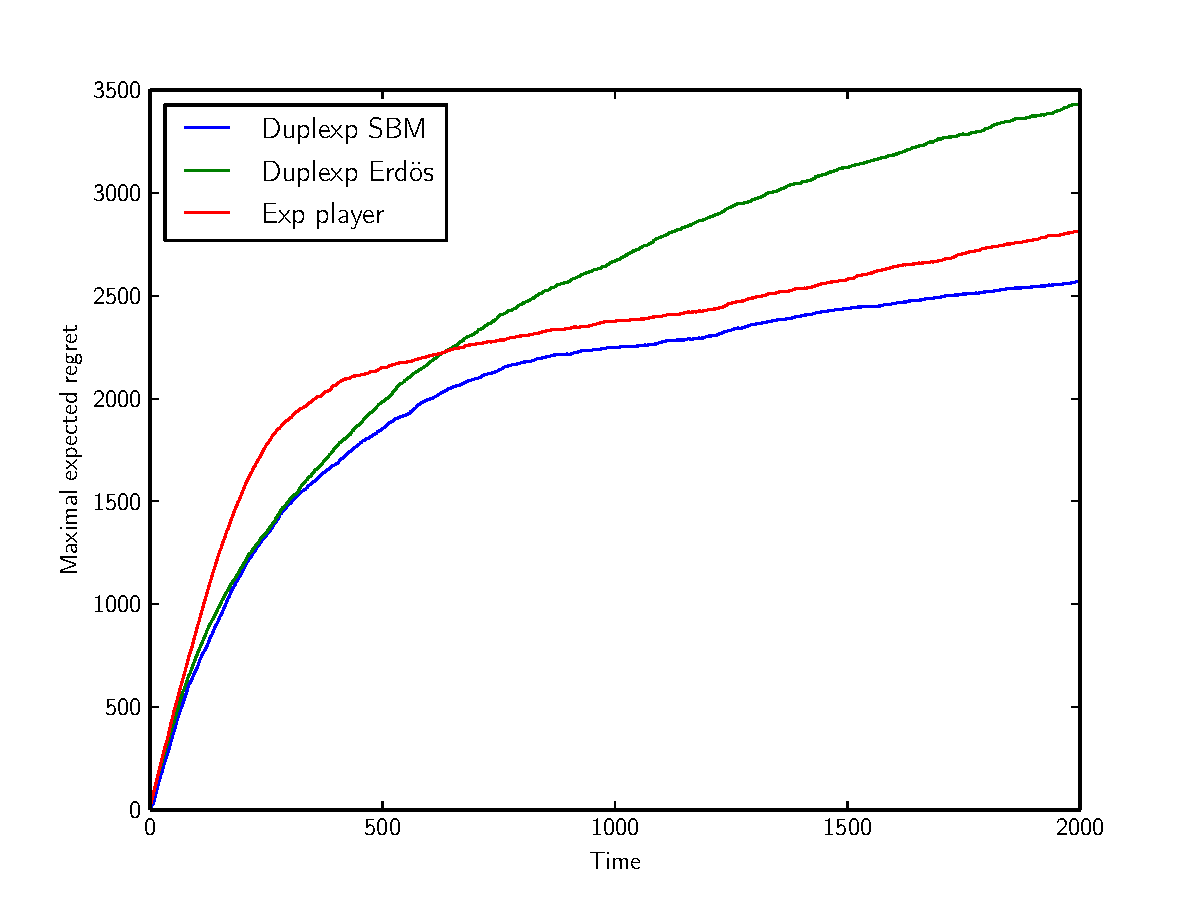
\includegraphics[width=0.8\textwidth]{hard}
	\caption{Outperformance of our algorithm}
	\label{fig:hard}
\end{figure}

\end{frame}

\begin{frame}{Graph 'close' to Erdös-Rényi}

\begin{figure}[ht]
	\centering
	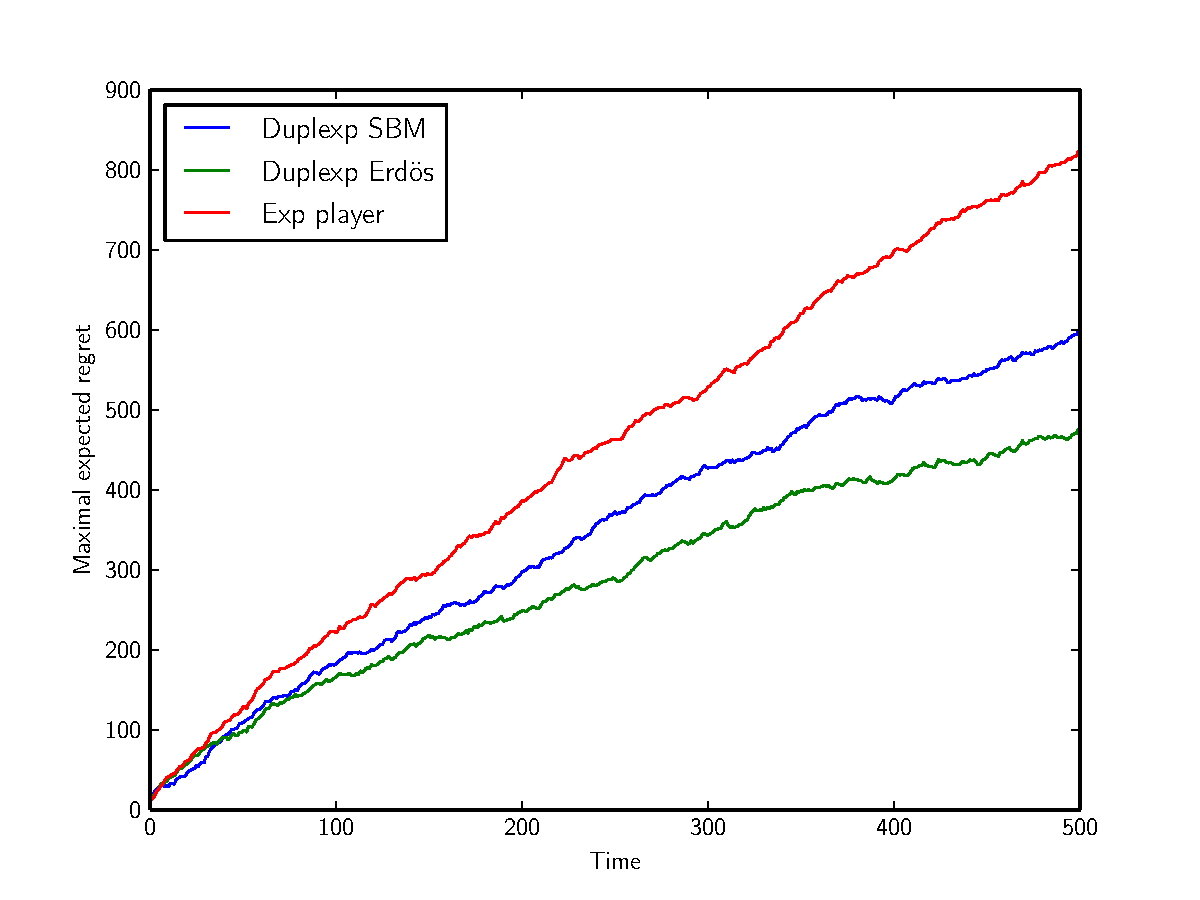
\includegraphics[width=0.8\textwidth]{easy}
	\caption{Orginal algorithm outperforms our algorithm}
	\label{fig:easy}
\end{figure}
\end{frame}

\end{document}